\section{PYTHIA 8.3}
\pythiaa{} \cite{pythia8300} è un generatore Monte Carlo utilizzato principalmente per la generazione di eventi di collisione di particelle nella fisica delle alte energie. 
Più in particolare esso riesce a riprodurre processi QCD utilizzando sia implementazioni teoriche che fenomenologiche, dove i parametri sono determinati a partire da dati sperimentali. 
L'utilizzo di \pythiaa{} può essere utile in molteplici campi, per esempio la maggior parte della base degli utenti proviene dalle grandi collaborazioni di LHC, ma anche in fisica astroparticellare oppure nucleare.

Per evento di collisione si intende l'insieme degli avvenimenti che comprendono le particelle iniziali, le particelle finali e tutte le particelle e risonanze intermedie.
La ripetizione nella generazione di questi eventi deve essere necessariamente resa casuale, data l'imprevedibilità dei processi quanto-meccanici.
La generazione dipende da parametri che vengono impostati nel software che possono essere modificati a piacimento dall'utente a seconda delle proprie esigenze.

\subsection{Struttura del programma}
% struttura di programma
In un vero evento di collisione di particelle vi sono numerosi processi QCD, QED e altri che sono noti per essere molto complessi, perciò è logico andare a ordinarli e raggrupparli secondo un criterio temporale o in termini di energie.
Per esempio in \cite{pythia8300} si prende come esempio un evento $pp\to t\bar t$ e si ordinano gli eventi secondo una logica in termini dell'\textit{hardness} dei processi:
si parte con uno scattering inelastico di partoni, seguito dalla produzione di risonanze (bosoni deboli o quark top), con aggiunta di correzioni radiative.
Successivamente si hanno radiazioni dello stato iniziale (ISR), e dello stato finale (FSR), originati dal decadimento delle particelle iniziali e dalle risonanze rispettivamente.
Queste radiazioni sono sostanzialmente sciami (o cascate) di partoni.
Contestualmente a ciò vi sono interazioni multi-partoniche (MPI), ulteriori processi di scattering, in aggiunta ad altri processi QCD che esulano dalla trattazione di questa tesi. 
Infine verso la fine del processo si formano gli adroni stabili a partire da decadimenti dei partoni instabili.
Una rappresentazione grafica di tutti questi processi è riportata in \autoref{fig:eventSchematic}.

\begin{figure}[htpb]
\centering % 73% + 27%
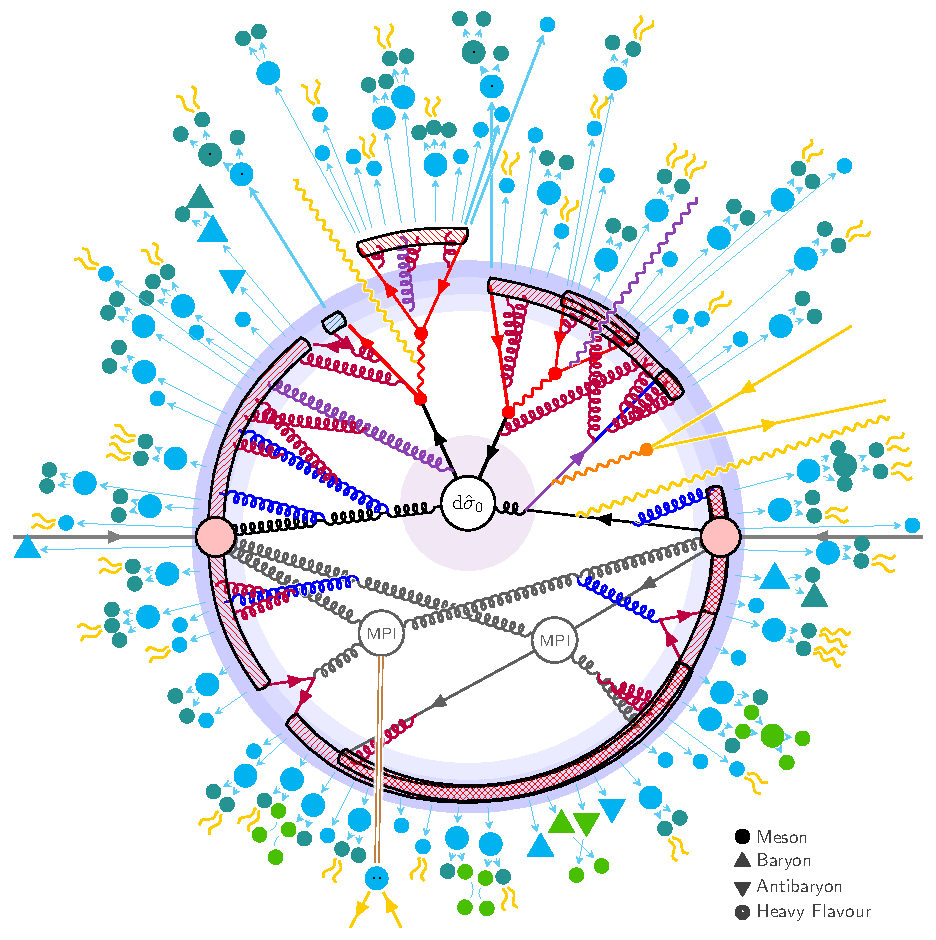
\includegraphics[width=0.73\textwidth]{image/2-modelli/event.pdf}%
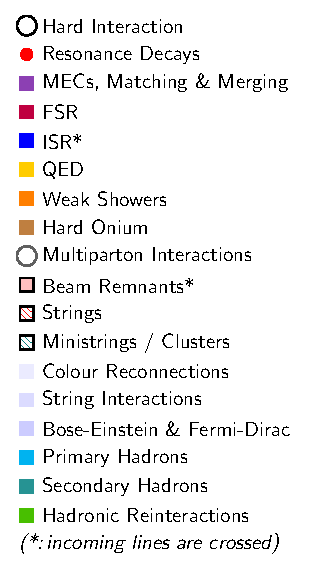
\includegraphics[width=0.27\textwidth]{image/2-modelli/eventLegend.pdf}
\captionwithsource{Schematica (semplificata) di un evento $pp\to t\bar t$ nel modello di \emph{\pythiaa{}}.
Le particelle entranti sono rappresentate dalle linee grigie esterne a metà altezza.  
\label{fig:eventSchematic}}{\cite{pythia8300}}
\end{figure}

\pythiaa{}, ispirandosi a questo modo di trattare un evento, è suddivisa in tre parti principali:
\begin{enumerate}
    \item \emph{livello di processo}, corrispettivo del processo di scattering duro, dove vengono prodotte anche le risonanze;
    \item \emph{livello di partoni}, dove vengono gestite le ISR e le FSR tramite l'implementazione di modelli di sciami partonici, le MPI e varie correzioni QCD;
    \item \emph{livello di adroni}, durante la quale viene gestita l'adronizzazione in senso stretto, tramite decadimenti di adroni e risonanze instabili e altri processi più tecnici.
\end{enumerate}
Ovviamente questi livelli non sono gestiti in maniera totalmente separata, ma vi è un numero significativo di oggetti condivisi da un livello all'altro.

% https://amzn.eu/d/6InjjKU per giovanni

\subsection{Gli algoritmi di generazione}
%%%%%%%%%%
Gli algoritmi di generazione in \pythiaa{} si basano su numeri pseudo-casuali campionati da distribuzioni di probabilità, simulando la natura stocastica degli eventi reali nelle collisioni di particelle.
In seguito vengono elencate le due principali utilizzate nel programma.
\begin{itemize}
    \item \emph{Algoritmo di veto}, il principale algoritmo di \pythiaa{} per simulare processi come decadimenti radiativi, cascate partoniche o interazioni multi-partoniche (MPI).
    Il suo funzionamento è semplice: partendo da una funzione di prova che sovrastima la distribuzione di probabilità desiderata, vengono generati dei campioni e viene deciso se sono conformi alla probabilità voluta, e in base a ciò viene deciso se la funzione di prova sia accettabile o se vi sia bisogno di ripetere questo step.
    Esistono inoltre anche varianti di questo algoritmo;
    % aggiungere altro se serve
    \item vi sono algoritmi per la distribuzione uniforme della quantità di moto nello spazio delle fasi.
    Nel caso di due particelle questo è triviale, in quanto è sufficiente emetterle in direzioni opposte nello spazio dei momenti.
    Mentre per tre o più particelle prodotte vengono utilizzate principalmente \emph{M-generator} e \emph{RAMBO}.
    Quest'ultimo è la migliore scelta per i prodotti senza massa (o massa trascurabile).
    \textit{M-generator} funziona scomponendo un processo di produzione  multiparticellare in produzione di 2 particelle.
    Per esempio un processo $0\to1234$ viene scomposto in $0\to(123) + 4$ e così via.
\end{itemize}
In generale, per ogni processo in \pythiaa{} è spesso implementata una forma derivata da uno di questi due principali algoritmi.   

\subsection{Formazione di deuteroni in PYTHIA} \label{ch:pythia_deuteron}
\pythiaa{} supporta la produzione deuteronica tramite due modelli di produzione, ovvero il modello di coalescenza e il modello di sezioni d'urto efficaci, chiamato anche modello di Dal-Raklev \cite{Dal_2015}, con quest'ultimo come opzione predefinita di \pythiaa{}.
Si noti come in questo paragrafo, per evitare ripetizioni, si tratterà solamente della produzione dei deuteroni, invece la trattazione degli antideuteroni è equivalente nel momento in cui si considerano le antiparticelle corrispettive.

\subsubsection{Modello di coalescenza}
Il modello di coalescenza, come già detto in precedenza, prevede la formazione di un deuterone nel momento in cui un protone e un neutrone sono sufficientemente vicini nello spazio delle fasi.
L'implementazione di questo modello in \pythiaa{} è effettuata in questo modo: vengono prese in considerazione tutte le coppie possibili di protoni e neutroni $p-n$ e si considera per ognuna di esse il modulo della differenza della loro quantità di moto (calcolato nel sistema di centro di massa di ognuna coppia)
\begin{equation}\label{eq:momentum_difference_k}
    k = |\vec p_p - \vec p_n|
\end{equation} 
Si determina la formazione del deuterone nel momento in cui $k<p_0$, con $p_0$ un parametro da determinare sperimentalmente.
È importante notare come non vi sia considerazione delle coordinate spaziali.
Un altro elemento da tenere in conto è la violazione energetica della coalescenza, ossia che il processo $pn\to D$ non è possibile se nello stato finale non vi sia un'altra particella.
Per ovviare a questo problema si considera al posto di questa reazione la cattura radiativa, ovvero $pn\to \gamma D$, in quanto provvede a fornire un'approssimazione ragionevole del processo.
Per esprimere la probabilità di formazione del deuterone in funzione di $k$ in modo compatto si può farlo nel seguente modo
\begin{equation}
    P(k) = \theta(p_0-k)
\end{equation}
con $\theta(k)$ la funzione gradino di Heaviside.

\subsubsection{Modello di sezioni d'urto efficaci}
Nel modello di sezioni d'urto efficaci si punta a descrivere la formazione dei deuteroni da un punto di vista probabilistico, di fatto considerando la probabilità di formazione $P_\text{processo}(k)$ direttamente proporzionale alla sezione d'urto differenziale del processo $\sigma_\text{processo}(k)$
\begin{gather}
    P_\text{processo}(k) \propto \dfrac{d\sigma_\text{processo}(k)}{dk} \\
    \implies P_\text{processo}(k) = \dfrac1{\sigma_0}\dfrac{d\sigma_\text{processo}(k)}{dk} 
\end{gather}
con $k$ la grandezza definita dell'\autoref{eq:momentum_difference_k} e $\sigma _0$ una costante di proporzionalità da determinare sperimentalmente, analogo di $p_0$.
L'obiettivo del modello di sezioni d'urto efficaci è anche quello di uniformare questo parametro in modo che sia costante in tutti gli esperimenti, al contrario di $p_0$ che assume valori diversi in esperimenti diversi. 

A differenza del modello di coalescenza, in questo modello non si considera solamente la reazione della cattura radiattiva, ma se ne considerano molteplici.
I canali di produzione dei deuteroni sono riportati in \autoref{tab:canali}.

\begin{table}[H]
    \centering
    \begin{tabular}{clcl}
    \hline \hline
    1) & $pn \to \gamma D$ & 5) & $pp \to \pi^+ D$\\
    2) & $pn \to \pi^0 D$ & 6) & $pp \to \pi^+\pi^0 D$\\
    3) & $pn \to \pi^-\pi^+ D$ & 7) & $nn \to \pi^- D$\\
    4) & $pn \to \pi^0\pi^0 D$ & 8) & $nn \to \pi^-\pi^0 D$\\
    \hline\hline
    \end{tabular}
    \caption{I canali di produzione dei deuteroni considerati nel modello di sezione d'urto. Per ottenere i canali dell'antideuterone è sufficiente considerare le antiparticelle.}
    \label{tab:canali}
\end{table}
Ognuno di questi canali ha una propria probabilità di formazione, determinata non più come una semplice distribuzione uniforme con cut-off come nel modello di coalescenza, ma determinata da fit di dati sperimentali sullo scattering differenziale di nucleoni.

Le possibili funzioni di sezioni d'urto differenziali ${d\sigma_\text{processo}(k)}/{dk}$ sono tre:
\begin{itemize}
    \item Per $pn\to\gamma D$ è parametrizzato da un polinomio sotto a un valore $a_0$ di $k$, altrimenti da un andamento esponenziale
    \begin{equation}
        \dfrac{d\sigma(k)}{dk} =
        \begin{cases}
            \displaystyle\sum_{i=1}^{12}a_ik^{i-2} & k<a_0 \\
            e^{-c_{13}k - c_{14}k} & k>a_0
        \end{cases}
    \end{equation}
    Si assume inoltre che per $k<0.1$ GeV la sezione d'urto differenziale sia fissata al valore di $k=0.1$ GeV.

    \item Per processi che coinvolgono la formazione di un pione e di un deuterone si assume la seguente forma della sezione d'urto differenziale
    \begin{equation}
        \dfrac{d\sigma(q)}{dq} = \dfrac{c_0\ q^{c_1}}{(c_2-e^{c_3 q})^2 + c_4}
    \end{equation}
    con $q = |\vec p_\pi|/m_\pi$, con $\vec p_\pi$ la quantità di moto del pione nel centro di massa e $m_\pi$ la massa del pione.

    \item Infine per i processi di formazione di 3 corpi la sezione d'urto differenziale è parametrizzata nel seguente modo
    \begin{equation}
        \dfrac{d\sigma(k)}{dk} = \sum_{i=0}\dfrac{c_{5i}\ k^{c_{1+5i}}}{(c_{2 + 5i}-e^{c_{3 + 5i} k})^2 + c_{4 + 5i}}
    \end{equation}
\end{itemize}
La giustificazione dell'utilizzo di queste forme delle sezioni d'urto è reperibile in \cite{Dal_2015}.\\

I valori dei parametri di coalescenza ($p_0$) e di Dal-Raklev sono già stati determinati eseguendo fit ai dati sperimentali e possono essere reperiti in \cite{Dal_2015}.
In \pythiaa{}, come è già stato detto, il modello predefinito è il modello di sezioni d'urto efficaci.
Il parametro $\sigma_0$, o meglio $1/\sigma_0$, è un parametro importante perché determina il numero di deuteroni prodotti in tutti i canali di produzione. 
Tuttavia, per ragioni pratiche, in \pythiaa{} il parametro $1/\sigma_0$ è incorporato in un altro parametro, ovvero \ttbox{DeuteronProduction:norm}, che per semplicità indicheremo con \ttbox{norm}, calcolato come 
\begin{equation}\label{eq:norm}
    \ttbox{norm} = \dfrac{1}{(1/\sigma_0)(d\sigma/dk)_\text{max}}
\end{equation}
con $(d\sigma/dk)_\text{max}$ il valore della sezione d'urto differenziale massima.
Il ruolo di questo parametro è simile a quello di $1/\sigma_0$, ossia quello di regolare il numero di (anti)deuteroni prodotti per tutti i canali. Più è alto il suo valore, minore è la produzione, e viceversa.\\

Usando i parametri della tabella VI di \cite{Dal_2015} è possibile ricavare il valore massimo della sezione d'urto differenziale che è di circa $3.18$ mb.
Perciò ora per ottenere il valore di \ttbox{norm} è sufficiente conoscere il valore di $1/\sigma_0$.
Tuttavia, la determinazione di questo parametro è problematica perché varia in base all'energia del centro di massa $\sqrt s$, e in \cite{Dal_2015} sono stati ottenuti i valori di $1/\sigma_0$ e di $p_0$ che vengono riportati nella tabella VIII in \cite{Dal_2015}, in base a fit effettuati sui dati di ALICE.
Questi valori sono riportati per convenienza in \autoref{tab:valori_p0_1sigma0}.
\begin{table}[H]
    \centering
    \begin{tabular}{||c||c|c||c|c||}
    \hline \hline
    & \multicolumn{2}{c||}{$p_0$ [\si{MeV}]} & \multicolumn{2}{c||}{$1/\sigma_0$ [\si{barn^{-1}}]}\\
    \hline
    \textsc{energia} & \textsc{deuteroni} & \textsc{antideut.} & \textsc{deuteroni} & \textsc{antideut.} \\ 
    \hline
    0.9 TeV & 201 & 201 & 3.58 & 3.63\\
    2.76 TeV & 194 & 196 & 2.93 & 2.88\\
    7 TeV & 194 & 195 & 2.63 & 2.58\\
    \hline\hline
    \end{tabular}
    \captionwithsource{I valori dei parametri $p_0$ e $1/\sigma_0$ alle energie riportate. Per \emph{\rmfamily\textsc{energia}} si intende l'energia  del centro di massa $\sqrt s$.}{\cite{Dal_2015}}
    \label{tab:valori_p0_1sigma0}
\end{table}
\pythiaa{} utilizza il parametro \ttbox{norm} considerando esclusivamente il valore di $1/\sigma_0$ a 7 \si{TeV} dei deuteroni, quindi, utilizzando l'\autoref{eq:norm}, si ha che $\ttbox{norm} = 119.6$.